\documentclass[10pt,a4paper]{article}
\usepackage[utf8]{inputenc}
\usepackage[spanish]{babel}
\usepackage{amsmath}
\usepackage{amsfonts}
\usepackage{amssymb}
\usepackage{makeidx}
\usepackage{graphicx}
\usepackage{listings}
\usepackage{color}
\usepackage{fancyhdr}
\usepackage[headheight=35pt]{geometry}

\begin{document}

\definecolor{gris claro}{gray}{0.97}
\definecolor{gris oscuro}{gray}{0.45}

\lhead{}
\rhead{\includegraphics[width=1.5cm]{captura03}}
\cfoot{}
\rfoot{\thepage}

\pagestyle{fancy}

\lstset{language=VBScript, frame=Ltb,
framerule=0pt,
aboveskip=0.5cm,
framextopmargin=3pt,
framexbottommargin=3pt,
framexleftmargin=0.4cm,
framesep=0pt,
rulesep=.4pt,
backgroundcolor=\color{gris claro},
rulesepcolor=\color{black},
%
stringstyle=\ttfamily,
showstringspaces = false,
basicstyle=\small\ttfamily,
commentstyle=\color{gris oscuro},
keywordstyle=\bfseries,
%
numbers=left,
numbersep=15pt,
numberstyle=\tiny,
numberfirstline = false,
breaklines=true,
}
\section*{Cálculo de la entalpía}

El presente documento sigue los lineamientos estipulados por la \textit{IAPWS} para las funciones de estado.\footnote{Acrónimo de \textit{``The International Association for the Properties of Water and Steam" .} Su formulación es el estándar para fines científicos y tecnológicos. Puede visitarse \texttt{http://www.iapws.org/} En caso de desearse la formulación completa, comunicarse con \texttt{pbarral@agrestsrl.com}}

\subsection*{Ingreso de variables}
Nuestro objetivo es obtener la expresión

\begin{equation}
h=h(p;T)
\end{equation}

La formulación está expresada de modo adimensional. Para ello, debemos calcular:

\begin{equation}
\pi=\frac{p}{p^*}
\end{equation}

siendo $p^*=1 \, M \! Pa$ y 

\begin{equation}
\tau=\frac{T^*}{T}
\end{equation}

con $T^*=540 \, K$. Por lo tanto, para que la formulación funcione, el ingreso de la presión y la temperatura debe hacerse en $M \! Pa$ y $K$, debiéndo realizarse las conversiones correspondientes.

\subsection*{Obtención de la entalpía}
La siguiente expresión sirve únicamente para vapor sobrecalentado, en los entornos normales de operación para un ciclo industrial.

La expresión que se utiliza es:

\begin{equation}
h(\pi;\tau)=RT \cdot \tau \cdot (\gamma_{\tau}^{\circ} + \gamma_{\tau}^{r})
\end{equation}

Siendo, $R=0,461\, 526 \,\frac{kJ}{kg \cdot K}$

Por su parte

\begin{equation}
\gamma_{\tau}^{\circ}=\sum_{i=1}^{9}n_i^{\circ} \cdot J_i^{\circ} \cdot \tau^{J_i^{\circ}-1} \label{Derivada parcial de la parte de gas ideal}
\end{equation}

Los coeficientes que deben usarse para la expresión (\ref{Derivada parcial de la parte de gas ideal}) son los siguientes:

\begin{figure}[hbtp]
\centering
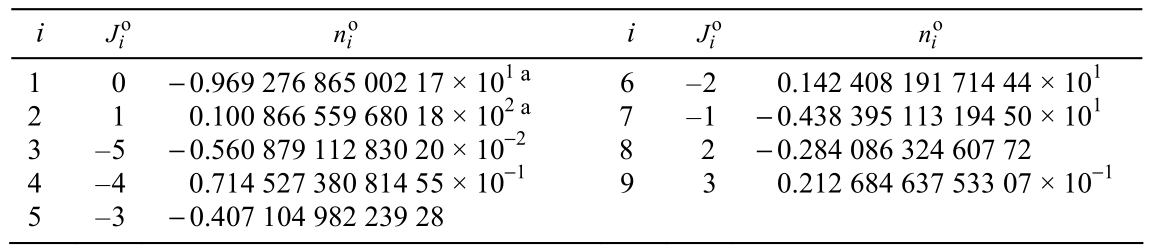
\includegraphics[scale=0.35]{Captura01.PNG}
\end{figure}

Finalmente,

\begin{equation}
\gamma_{\tau}^{r} = \sum_{i=1}^{43} n_i \cdot \pi^{I_i} \cdot J_i \cdot (\tau-0.5)^{J_i-1} \label{Derivada parcial de la parte residual}
\end{equation}

Los coeficientes que deben usarse para la expresión (\ref{Derivada parcial de la parte residual}) son los siguientes:

\begin{figure}[hbtp]
\centering
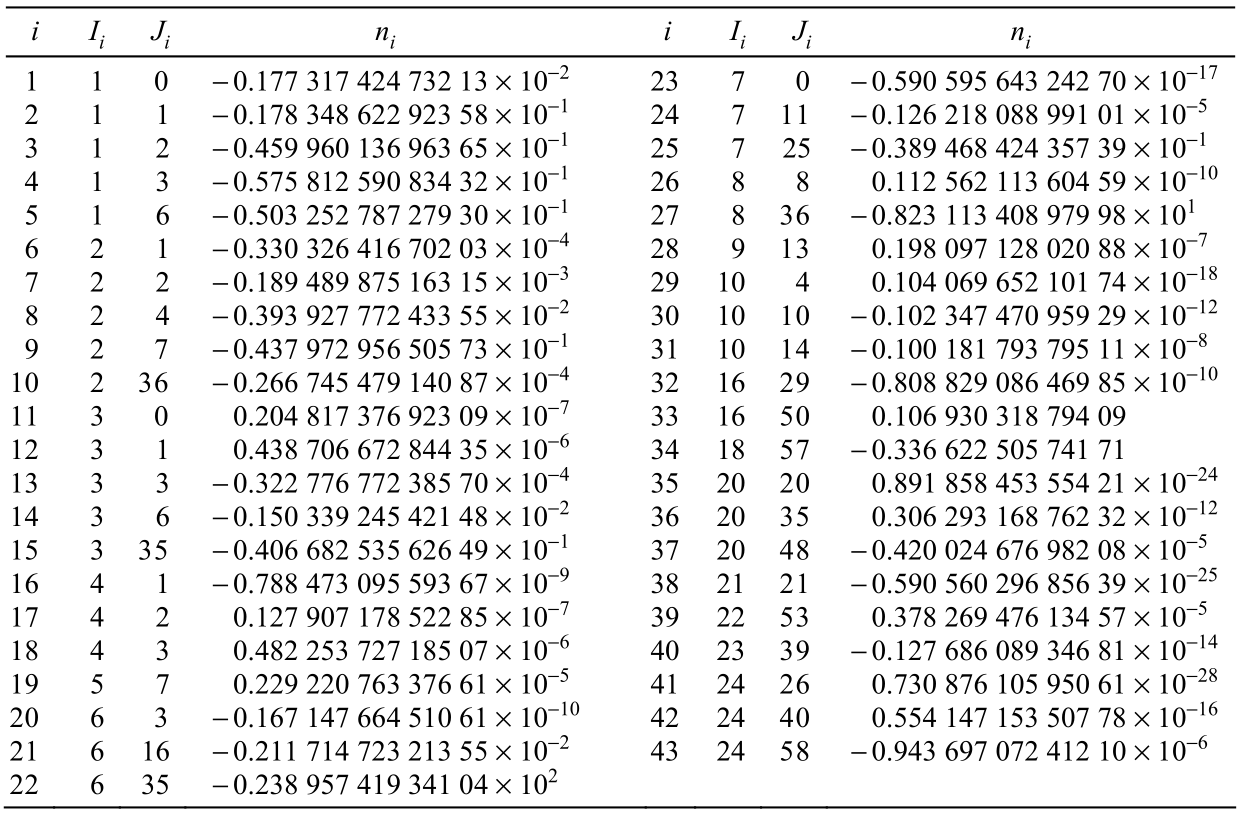
\includegraphics[scale=0.35]{Captura02.PNG}
\end{figure}

\subsection*{Líneas de comando en Visual Basic}

Las siguientes líneas funcionan como \textit{macro} en MS Excel. Adaptando la sintaxis, puede utilizarse en cualquier lenguaje de programación.

%https://en.wikibooks.org/wiki/LaTeX/Source_Code_Listings
\begin{lstlisting}
Function h2_pT(ByVal p As Double, ByVal T As Double) As Double
'Release on the IAPWS Industrial Formulation 1997 for the Thermodynamic Properties of Water and Steam, September 1997
'6 Equations for Region 2, Section. 6.1 Basic Equation
'Table 11 and 12, Page 14 and 15
  Dim i As Integer
  Dim tau, g0_tau, gr_tau As Double
  Dim Ir, Jr, nr, J0, n0 As Variant
  Const R As Double = 0.461526 'kJ/(kg K)
  J0 = Array(0, 1, -5, -4, -3, -2, -1, 2, 3)
  n0 = Array(-9.6927686500217, 10.086655968018, -0.005608791128302, 0.071452738081455, -0.40710498223928, 1.4240819171444, -4.383951131945, -0.28408632460772, 0.021268463753307)
  Ir = Array(1, 1, 1, 1, 1, 2, 2, 2, 2, 2, 3, 3, 3, 3, 3, 4, 4, 4, 5, 6, 6, 6, 7, 7, 7, 8, 8, 9, 10, 10, 10, 16, 16, 18, 20, 20, 20, 21, 22, 23, 24, 24, 24)
  Jr = Array(0, 1, 2, 3, 6, 1, 2, 4, 7, 36, 0, 1, 3, 6, 35, 1, 2, 3, 7, 3, 16, 35, 0, 11, 25, 8, 36, 13, 4, 10, 14, 29, 50, 57, 20, 35, 48, 21, 53, 39, 26, 40, 58)
  nr = Array(-1.7731742473213E-03, -0.017834862292358, -0.045996013696365, -0.057581259083432, -0.05032527872793, -3.3032641670203E-05, -1.8948987516315E-04, -3.9392777243355E-03, -0.043797295650573, -2.6674547914087E-05, 2.0481737692309E-08, 4.3870667284435E-07, -3.227767723857E-05, -1.5033924542148E-03, -0.040668253562649, -7.8847309559367E-10, 1.2790717852285E-08, 4.8225372718507E-07, 2.2922076337661E-06, -1.6714766451061E-11, -2.1171472321355E-03, -23.895741934104, -5.905956432427E-18, -1.2621808899101E-06, -0.038946842435739, 1.1256211360459E-11, -8.2311340897998, 1.9809712802088E-08, 1.0406965210174E-19, -1.0234747095929E-13, -1.0018179379511E-09, -8.0882908646985E-11, 0.10693031879409, -0.33662250574171, 8.9185845355421E-25, 3.0629316876232E-13, -4.2002467698208E-06, -5.9056029685639E-26, 3.7826947613457E-06, -1.2768608934681E-15, 7.3087610595061E-29, 5.5414715350778E-17, -9.436970724121E-07)
  tau = 540 / T
  g0_tau = 0#
  For i = 0 To 8
    g0_tau = g0_tau + n0(i) * J0(i) * tau ^ (J0(i) - 1)
  Next i
  gr_tau = 0#
  For i = 0 To 42
   gr_tau = gr_tau + nr(i) * p ^ Ir(i) * Jr(i) * (tau - 0.5) ^ (Jr(i) - 1)
  Next i
  h2_pT = R * T * tau * (g0_tau + gr_tau)
End Function
\end{lstlisting}
\end{document}
